\documentclass[a4paper]{article}

%% Language and font encodings
\usepackage[english]{babel}
\usepackage[utf8x]{inputenc}
\usepackage[T1]{fontenc}


%% Sets page size and margins
\usepackage[a4paper,top=3cm,bottom=2cm,left=3cm,right=3cm,marginparwidth=1.75cm]{geometry}

%% Useful packages
\usepackage{amsmath}
\usepackage{graphicx}
\usepackage[colorinlistoftodos]{todonotes}
\usepackage[colorlinks=true, allcolors=blue]{hyperref}

\title{Actividad IX}
\author{Jose Pablo Montaño De la Ree}

\begin{document}
\maketitle



\section{Introduccion}

WXMaxima es un sistema computacional de algenra, que recive comandos de una forma similar a la que el usuario escribiria estas ecuaciones y trata de dar resultados como el usuario los esperaria. Este sistema fue diseñado por el MIT en la decada de los 60 y para 1980 el codigo fue puesto en varias plataformas. 

\section{Entrada y salida de datos}

Pra introducir datos en WXmaxima, se inicia por ( $\%$ i1 ), escrito ya por el ordenador donde i se refiere a input, despues se procede a dar una instruccion seguida por un ";". Al dar enter se guarda ahi la variable y se simplifica. Para llamarla se da shift + enter y la computadora contesta  escribe en el ordenador  ( $\%$ o1 ) donde o se refiere a output.





\section{Como integrar en wxMaximan}

Para integrar en wxMaxima lo primero que hay que saber es como hablar con el ordenador y pedrile que integre. Para esto se da el comando "integrate("1","2")", donde en "1" escribes la funcion a intehrar y en "2" escribes respecto a que variable. A continuacion un ejemplo. 
\linebreak
Integre $x/x^2$ respecto a X.


\begin{figure}[ht!]
\centering
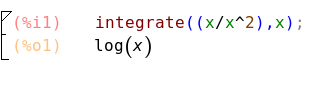
\includegraphics[width=0.3\textwidth]{1.png}
\caption{\label{fig:}}
\end{figure}


Recordemos que tambien existen funciones intrinsicas que nos pueden ayudar para sinX cosX etc. A continuacion se muestra una tabla que muestra estas funciones y su descripcion.
\newpage

\begin{figure}[ht!]
\centering
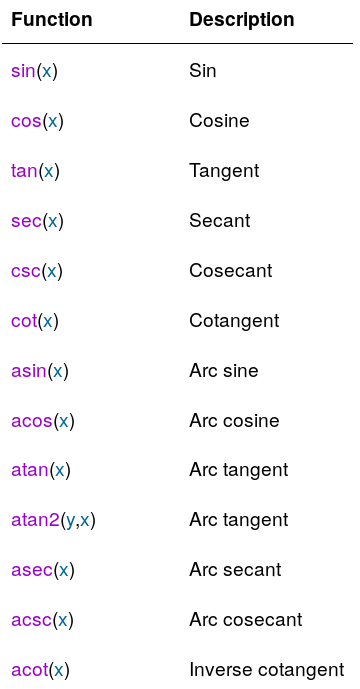
\includegraphics[width=0.3\textwidth]{2.png}
\caption{\label{fig:}}
\end{figure}

Ahora bien realicemos un pequeño ejemplo. Integremos la funcion $sin(x)cos(x)$ respecto a X.

\begin{figure}[ht!]
\centering
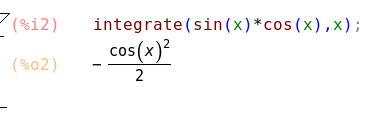
\includegraphics[width=0.3\textwidth]{3.png}
\caption{\label{fig:}}
\end{figure}

Ahora bien, recordemos que las intehrales tambien pueden estar definidas dentro de ciertos limites. Para comandar una integral con limites utilice el comandon "integrate("1","2","3","4")", donde "1" es la funcion a integrar, "2" respecto a que variable, "3" el limite inferior y "4" el limite superior. 
\linebreak
Realizemos ahora el siguiente ejemplo. Integre la funcion $3x^2+3$ respecto a x con limite inferior 0 y limite superior 1.

\begin{figure}[ht!]
\centering
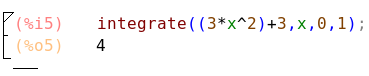
\includegraphics[width=0.3\textwidth]{4.png}
\caption{\label{fig:}}
\end{figure}

Las integrales, no solo son respecto a una sola variable o respecto a a la variable que se encuentra en el integrando. Intentemos para una exploracion primaria la integral de x respecto a y.

\begin{figure}[ht!]
\centering
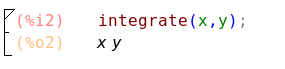
\includegraphics[width=0.3\textwidth]{5.png}
\caption{\label{fig:}}
\end{figure}
 Tambien es posible darle a estas integrales limites definidos. Realizemos el ejercisio anterior pero con limites de 0 a 1.
\newpage
 

\begin{figure}[ht!]
\centering
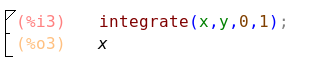
\includegraphics[width=0.3\textwidth]{6.png}
\caption{\label{fig:}}
\end{figure} 

De igual forma que se le pueden dar limites definidos, se le pueden dar limites en forma de otras variables. Realizemos el ejercisio anterior con limites de 0 a (x+1).


\begin{figure}[ht!]
\centering
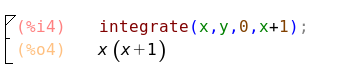
\includegraphics[width=0.3\textwidth]{7.png}
\caption{\label{fig:}}
\end{figure}

De los ejercisios anteriores podemos concluior de que es posible realizar integrales iteradas en wMaxima. Intentemos hacer la integral iterada de x respecto a y con limites [0,x+1] y respecto a x con limites [0,1]. Intentemoslo primero escribiendo dos veces el comando integrate y colocando dentro de los primeros parentesis los limites de y y dentro de los segundos los limites de x como se muestra acontinuacion. 

\begin{figure}[ht!]
\centering
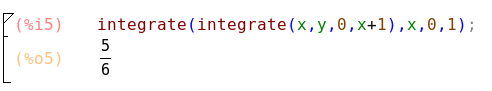
\includegraphics[width=0.3\textwidth]{8.png}
\caption{\label{fig:}}
\end{figure}

Notese que se pude obtener el mismo resultado si se realiza la integral por separado, es decir, primero integrando respecto a y, para despues integrar respecto a x asignando la funcion a integrar con el nombre que da wxMaxima al resultado $\%$ num.

\begin{figure}[ht!]
\centering
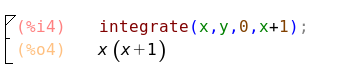
\includegraphics[width=0.3\textwidth]{7.png}
\caption{\label{fig:}}
\end{figure}


\begin{figure}[ht!]
\centering
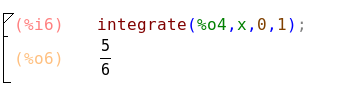
\includegraphics[width=0.3\textwidth]{9.png}
\caption{\label{fig:}}
\end{figure}

De esto podemos colcluir que es posible realizar integrales iteradas tan complicadas como deseemos y resolverlas con wxmaxima. 
\newpage
\section{Ejercisio}

Integre la esfera unitaria $x^2+y^2+z^2=1$

Para realizar esta integral es necesario definir los limites. 
$0<x<1, -sqrt(1-x^2)<y<sqrt(1-x^2), -sqrt(1-x^2-y^2) <z< sqrt(1-x^2-y^2)$ 
\linebreak
Despues integramos usando la funcion integrate de wxmaxima, recordando que como queremos integrar respecto a dz,dy,dx, pondremos en el area del integarndo un 1, para que al multiplicarse por los diferenciales de los diferenciales. 
\linebreak
Tomando en consideracion el tamaño de los limites, integraremos un diferencial a la vez. 

\begin{figure}[ht!]
\centering
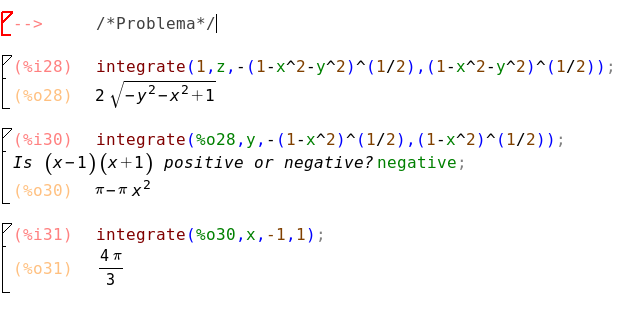
\includegraphics[width=0.7\textwidth]{10.png}
\caption{\label{fig:}}
\end{figure}

\section{Apendice}

    ¿Cuál fue tu primera impresión de wxmaxima?
    \linebreak
    Que puede realizar calculos complejos rapidamente ahorrandome mucho tiempo.
    \linebreak
    ¿Crees que esta herramienta puede ser útil en otros de tus cursos?
    \linebreak
    Totalmente, podria ser muy util para calculo, electromagnetismo y mecanica teorica.
    \linebreak
    ¿Qué se te dificultó mas en esta actividad?
    \linebreak
    aprender como hablar con wxmaxima, los pequeños errores daban resultados fuera de lo esperado.
    \linebreak
    ¿Se te hizo compleja esta actividad? ¿Cómo la mejorarías? 
    \linebreak
    Un poco, la mejoraria con una clase de introduccion. 

\end{document}